% !TEX root = ../main.tex
\section{Perceptual Ambiguity}
\label{sec:problem}
In most square fiducial tag detection, the pose of the tag is calculated from the quad fitted around the tag. The corners are extracted from the tag and the pose of the tag is estimated using some 3D to 2D point correspondence optimization. However, small variance in the corner detection process will yield estimations far from the true pose due to a perceptual ambiguity under perspective projection. 

We will illustrate this effect by using two over lapping cubes in figure 3. The marked face of both cubes are interlaced and oriented off by 120 degrees. However, due to perspective projection the squares appears to be on the same plane. Note that in theory, the perfect (Back this up with formula) perspective projection of a square should be unique. However, the projected square of the above set up are close to each other. Therefore, under noise, the two projected squares become indistinguishable. The result of the 3D to 2D correspondence optimization might return either one of the two solution.
\begin{figure}
\centering
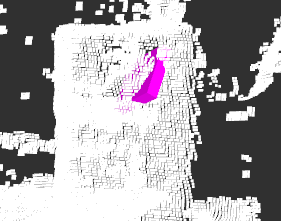
\includegraphics[width=\columnwidth]{figs/mismatch_tag}
\caption{The orientation of Apriltag placed on the object is greatly misaligned with the actual object}
\label{fig:calib}
\end{figure}

\begin{figure}
\centering
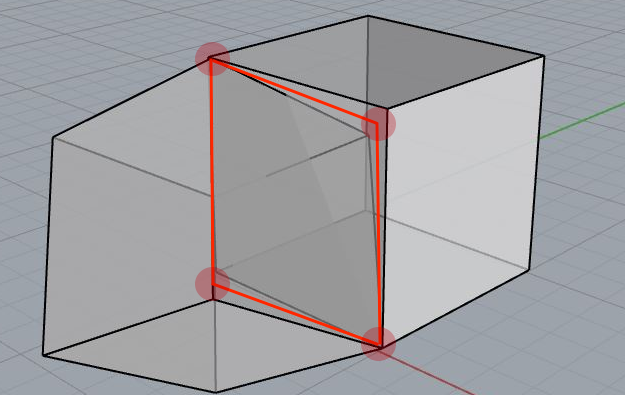
\includegraphics[width=\columnwidth]{figs/perspective_fig}
\caption{Perspective Ambiguity illustrated with overlapping cubes}
\label{fig:calib}
\end{figure}